\documentclass{amsart}
\title[The Dynkin diagrams package]%
{The Dynkin diagrams package \\ 
Version 3.141\,592\,653\,589\,793\,238\,4}
%% My name:
\makeatletter
\DeclareRobustCommand{\scotsMc}{\scotsMcx{c}}
\DeclareRobustCommand{\scotsMC}{\scotsMcx{\textsc{c}}}
\DeclareRobustCommand{\scotsMcx}[1]{%
  M%
  \raisebox{\dimexpr\fontcharht\font`M-\height}{%
    \check@mathfonts\fontsize{\sf@size}{0}\selectfont
    \kern.3ex\underline{\kern-.3ex #1\kern-.3ex}\kern.3ex
  }%
}
\expandafter\def\expandafter\@uclclist\expandafter{%
  \@uclclist\scotsMc\scotsMC
}
\makeatother
\author{Ben \scotsMc{}Kay}
\address{School of Mathematical Sciences,  University College Cork, Cork, Ireland}
\email{b.mckay@ucc.ie}
\date{2 June 2023}
\usepackage[T1]{fontenc}
\usepackage[utf8]{inputenx}
\usepackage{etoolbox} 
\usepackage{lmodern}
\RequirePackage[tt={lining=true,variable=false}]{cfr-lm}
\usepackage[kerning=true,tracking=true]{microtype}
\usepackage{amsmath}
\usepackage{amsfonts}
\usepackage{mathtools}
\usepackage{array}
\usepackage{xstring}
\usepackage{longtable}
\usepackage[dvipsnames,table]{xcolor}
\usepackage[listings]{tcolorbox} 
\tcbuselibrary{breakable}
\tcbuselibrary{skins}
\usepackage[pdftex]{hyperref}
\hypersetup{
  colorlinks   = true,  %Colours links instead of ugly boxes
  urlcolor     = black, %Colour for external hyperlinks
  linkcolor    = black, %Colour of internal links
  citecolor    = black  %Colour of citations
}
\usepackage{booktabs}
\usepackage{colortbl}
\usepackage{varwidth}
\usepackage{dynkin-diagrams}
\usepackage{fancyvrb}
\usepackage{xspace}
\newcommand{\TikZ}{Ti\textit{k}Z\xspace}
\usetikzlibrary{decorations.markings}
\usetikzlibrary{decorations.pathmorphing}
\usepackage{tikz-cd}
%% Use white rulings in tables.
\arrayrulecolor{white}
\makeatletter
    \def\rulecolor#1#{\CT@arc{#1}}
    \def\CT@arc#1#2{%
      \ifdim\baselineskip=\z@\noalign\fi
      {\gdef\CT@arc@{\color#1{#2}}}}
    \let\CT@arc@\relax
\rulecolor{white}
\makeatother

\newcommand{\C}[1]{\mathbb{C}^{#1}}
\renewcommand*{\arraystretch}{1.5}
\newcommand{\wdtA}{.7cm}
\newcommand{\wdtD}{3cm}
\newcommand{\wdtE}{6cm}
\newcommand{\wdtL}{3cm}
\newcolumntype{A}{@{}>{\columncolor[gray]{.9}$}m{\wdtA}<{$}} 
\newcolumntype{B}{@{}>{\columncolor[gray]{.9}}m{\wdtA}} 
\newcolumntype{D}{>{\columncolor[gray]{.9}}m{\wdtD}}
\newcolumntype{E}{>{\columncolor[gray]{.9}}m{\wdtE}}
\newcolumntype{L}{>{\columncolor[gray]{.9}}p{\wdtL}}
\newcolumntype{M}{>{\columncolor[gray]{.9}}l}
\newcolumntype{P}{>{\columncolor[gray]{.9}}p{10cm}}
\NewDocumentCommand\textleftcurly{}{\texttt{\char'173}}%
\NewDocumentCommand\textrightcurly{}{\texttt{\char'175}}%
\newcount\seriesLength
\newcount\rankLength
\NewDocumentCommand\csDynkin{omom}%
{%
	\texttt{\detokenize{\dynkin}\!\!%
	\IfNoValueTF{#1}{}{[#1]}%
	\StrLen{#2}[\thatseriesLength]%
	\seriesLength\thatseriesLength\relax%
	\ifnum\seriesLength=1\relax%
		\IfNoValueT{#1}{\ }%
		#2%
	\else%
		\textleftcurly#2\textrightcurly%
	\fi%
	\IfNoValueTF{#3}{}{[#3]}%
	\StrLen{#4}[\thatrankLength]%
	\rankLength\thatrankLength\relax%
	\ifnum\rankLength=1\relax%
		#4%
	\else%
		\textleftcurly#4\textrightcurly%
	\fi%
	}%
}%

\NewDocumentCommand\dynk{omom}%
{%
	\dynkin[#1]{#2}[#3]{#4}&\csDynkin[#1]{#2}[#3]{#4}\\
}%

\NewDocumentCommand\typesetSubseries{m}%
{%
	\IfInteger{#1}{#1}{\IfStrEq{#1}{}{n}{#1}}
}%

\NewDocumentCommand\dyn{omom}%
{%
	{#2}_{\typesetSubseries{#4}}^{\IfInteger{#3}{#3}{\IfStrEq{#1}{extended}{1}{}}} & \dynk[#1]{#2}[#3]{#4}%
}%


\NewDocumentEnvironment{dynkinTable}{mmm}%
{%
\renewcommand{\wdtD}{#2}
\renewcommand{\wdtL}{#3}
\begin{longtable}{ADM}
\caption{#1}\\
\endfirsthead
\caption{\dots continued}\\
\endhead
\multicolumn{2}{c}{continued \dots}\\
\endfoot
\endlastfoot
}%
{%
\end{longtable}
}%


\definecolor{example-color}{gray}{.85}
\definecolor{example-border-color}{gray}{.7} 

\tcbset{coltitle=black,colback=example-color,colframe=example-border-color,enhanced,breakable,pad at break*=1mm,
toprule=1.2mm,bottomrule=1.2mm,leftrule=1mm,rightrule=1mm,toprule at break=-1mm,bottomrule at break=-1mm,
before upper={\widowpenalties=3 10000 10000 150}}

\makeatletter
\def\@tocline#1#2#3#4#5#6#7{\relax
  \ifnum #1>\c@tocdepth%
  \else
    \par \addpenalty\@secpenalty\addvspace{#2}%
    \begingroup \hyphenpenalty\@M
    \@ifempty{#4}{%
      \@tempdima\csname r@tocindent\number#1\endcsname\relax
    }{%
      \@tempdima#4\relax
    }%
    \parindent\z@ \leftskip#3\relax \advance\leftskip\@tempdima\relax
    #5\leavevmode\hskip-\@tempdima #6\nobreak\relax
    ,~#7\par
    \endgroup
  \fi}
\makeatother

\fvset{fontsize=\small,tabsize=4}

\begin{document}
\maketitle
\begin{center}
\begin{varwidth}{\textwidth}
\tableofcontents
\end{varwidth}
\end{center}

\setlength{\arrayrulewidth}{1.5pt}

\section{Quick introduction}
\begin{tcolorbox}[title={Load the Dynkin diagram package (see options below)}]
\begin{Verbatim}
\documentclass{amsart}
\usepackage{dynkin-diagrams} 
\begin{document}
The Dynkin diagram of \(B_3\) is \dynkin B3.
\end{document}
\end{Verbatim}
\end{tcolorbox}
\begin{tcblisting}{title={Invoke it}}
The Dynkin diagram of \(B_3\) is \dynkin B3.
\end{tcblisting}
\begin{tcblisting}{title={Indefinite rank Dynkin diagrams}}
\dynkin B{}
\end{tcblisting}
\begin{tcblisting}{title={Inside a \TikZ statement}}
The Dynkin diagram of \(B_3\) is 
\tikz \dynkin B3;
\end{tcblisting}
\begin{tcblisting}{title={Inside a Dynkin diagram environment}}
The Dynkin diagram of \(B_3\) is 
\begin{dynkinDiagram}B3
\draw[very thick,red] (root 1) to [out=-45, in=-135] (root 3);
\end{dynkinDiagram}
\end{tcblisting}
\newpage
\section{Interaction with \TikZ}
Inside a \TikZ environment, default behaviour is to draw from the origin, so you can draw around the diagram:
\begin{tcblisting}{title={Inside a \TikZ environment}}
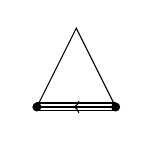
\begin{tikzpicture}
\draw (0,0) -- (.5,1) -- (1,0);
\dynkin[edge length=1cm]G2
\end{tikzpicture}
\end{tcblisting}
But it looks bad in the middle of text:
\begin{tcblisting}{title={Inside a \TikZ environment}}
The Dynkin diagram of \(B_3\) is 
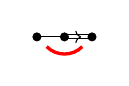
\begin{tikzpicture}[baseline]
\dynkin B3
\draw[very thick,red] (root 1) to [out=-45, in=-135] (root 3);
\end{tikzpicture}
\end{tcblisting}
A vertical shift realigns the diagram to ambient text:
\begin{tcblisting}{title={Inside a \TikZ environment}}
The Dynkin diagram of \(B_3\) is 
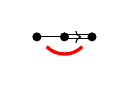
\begin{tikzpicture}[baseline]
\dynkin[vertical shift] B3
\draw[very thick,red] (root 1) to [out=-45, in=-135] (root 3);
\end{tikzpicture}
\end{tcblisting}

\newpage 

\renewcommand\do[1]{\dyn#1}
\renewcommand{\wdtA}{3cm}
\begin{dynkinTable}{The Dynkin diagrams of the reduced simple root systems \cite{Bourbaki:2002} pp. 265--290, plates I--IX}{2.25cm}{2.5cm}
\docsvlist{A{},B{},C{},D{},E6,E7,E8,F4,G2}
\end{dynkinTable}


\section{Set options globally}

\begin{tcolorbox}[title={Most options set globally \dots}]
\begin{Verbatim}
\pgfkeys{/Dynkin diagram,
	edge length=.5cm,
	fold radius=.5cm,
	indefinite edge/.style={
    	draw=black,
    	fill=white,
    	thin,
    	densely dashed}}
\end{Verbatim}
\end{tcolorbox}
You can also pass options to the package in \verb!\usepackage!.
\emph{Danger:} spaces in option names are replaced with hyphens: \texttt{edge length=1cm} is \texttt{edge-length=1cm} as a global option; moreover you should drop the extension \verb!/.style! on any option with spaces in its name (but not otherwise). For example,
\begin{tcolorbox}[title={\dots or pass global options to the package}]
\begin{Verbatim}
\usepackage[
     ordering=Kac,
     edge/.style=blue,
	 indefinite-edge={draw=green,fill=white,densely dashed},
	 indefinite-edge-ratio=5,
     mark=o,
     root-radius=.06cm]
     {dynkin-diagrams}
\end{Verbatim}
\end{tcolorbox}

\section{Disconnected Dynkin diagrams}
Disconnected Dynkin diagrams that represent a product of simple Lie groups (or a sum of Lie algebras, or a product of Coxeter systems, \dots) have a different syntax (to ensure back compatibility):
\begin{tcblisting}{title={Command}}
The Dynkin diagram of \(B_3 \times A_2\) is \dynkins{B3|A2}.
\end{tcblisting}
\begin{tcblisting}{title={Environment}}
The Dynkin diagram of \(B_3 \times A_2\) is 
\begin{DynkinDiagrams}{B3|A2}\end{DynkinDiagrams}
\end{tcblisting}
Each factor can have its own options.
\begin{tcblisting}{title={Environment}}
The Dynkin diagram of \(B_3 \times A_2\) is 
\[
\begin{DynkinDiagrams}{[name=Bob]B3|[name=Alice]A2}
\draw[very thick,blue] (Bob root 1) 
  to [out=-45, in=-135] (Alice root 2);
\end{DynkinDiagrams}
\]
\end{tcblisting}
They are spaced out by the length of one edge between successive diagrams; change this with \texttt{separator length}.
\begin{longtable}{@{}>{\columncolor[gray]{.9}$}m{1.5cm}<{$}%
@{}>{\columncolor[gray]{.9}$}m{1cm}<{$}%
@{}>{\columncolor[gray]{.9}$}m{3cm}<{$}}
\caption{The Dynkin diagrams of the rank $2$ root systems}\\
\endfirsthead
\caption{\dots continued}\\
\endhead
\multicolumn{2}{c}{continued \dots}\\
\endfoot
\endlastfoot
A_1\times A_1&\dynkins{A1|A1}&\texttt{\detokenize{\dynkins}\{A1|A1\}}\\
A_2&\dynkins{A2}&\texttt{\detokenize{\dynkins}\{A2\}}\\
B_2&\dynkins{B2}&\texttt{\detokenize{\dynkins}\{B2\}}\\
C_2&\dynkins{C2}&\texttt{\detokenize{\dynkins}\{C2\}}\\
D_2&\dynkins{D2}&\texttt{\detokenize{\dynkins}\{D2\}}\\
G_2&\dynkins{G2}&\texttt{\detokenize{\dynkins}\{G2\}}\\
\end{longtable}

\section{Coxeter diagrams}

\begin{tcblisting}{title={Coxeter diagram option}}
\dynkin[Coxeter]F4
\end{tcblisting}

\begin{tcblisting}{title={gonality option for \(G_2\) and \(I_n\) Coxeter diagrams}}
\(G_2=\dynkin[Coxeter,gonality=n]G2\), \ 
\(I_n=\dynkin[Coxeter,gonality=n]I{}\)
\end{tcblisting}

\renewcommand\do[1]{\dyn#1}
\begin{dynkinTable}{The Coxeter diagrams of the simple reflection groups}{2.25cm}{6cm}
\forDynkinSemicolonsvlist{\do}{
[Coxeter]A{};
[Coxeter]B{};
[Coxeter]C{};
[Coxeter]D{};
[Coxeter]E6;
[Coxeter]E7;
[Coxeter]E8;
[Coxeter]F4;
[Coxeter,gonality=n]G2;
[Coxeter]H2;
[Coxeter]H3;
[Coxeter]H4;
[Coxeter,gonality=n]I{}}
\end{dynkinTable}

\section{Satake diagrams}\label{section:Satake}
\begin{tcblisting}{title={Satake diagrams use the standard name instead of a rank}}
\(A_{IIIb}=\dynkin A{IIIb}\)
\end{tcblisting}

We use a solid gray bar to denote the folding of a Dynkin diagram, rather than the usual double arrow, since the diagrams turn out simpler and easier to read.

\renewcommand\do[1]{\dyn#1}
\begin{dynkinTable}{The Satake diagrams of the real simple Lie algebras \cite{Helgason:2001} p. 532--534}{2.75cm}{3cm}
\docsvlist{A{I},A{II},A{IIIa},A{IIIb},A{IV},B{I},B{II},C{I},C{IIa},C{IIb},
D{Ia},D{Ib},D{Ic},D{II},D{IIIa},D{IIIb},
E{I},E{II},E{III},E{IV},E{V},E{VI},E{VII},E{VIII},E{IX},F{I},F{II},GI}
\end{dynkinTable}

\section{How to fold}
\begin{tcblisting}{title={If you don't like the solid gray ``folding bar'', most people use arrows. Here is \(E_{II}\)}}
\dynkin[edge length=.75cm,
        labels*={1,...,6},
        involutions={16;35}]E6
\end{tcblisting}

\begin{tcblisting}{title={The double arrows for \(A_{IIIa}\) are big}}
\dynkin[edge length=.75cm,
        involutions={1{10};29;38;47;56}]{A}{oo.o**.**o.oo}
\end{tcblisting}

\newpage

\begin{tcblisting}{title={We can add labels}}
\dynkin[edge length=.75cm,
    involutions={
        1<below>[\sigma]{10};
        2<below>[\sigma]9;
        3<below>[\sigma]8;
        4<below>[\sigma]7;
        5<below>[\sigma]6}
]{A}{oo.o**.**o.oo}
\end{tcblisting}

\begin{tcblisting}{title={Style options}}
\dynkin[edge length=.75cm,
	    involution/.style={blue!50,stealth-stealth,thick},
        involutions={1{10};29;38;47;56}
       ]{A}{oo.o**.**o.oo}
\end{tcblisting}

\begin{tcblisting}{title={Arrow angles}}
\dynkin[edge length=.75cm,
        involutions={[in=-120,out=-60,relative]1{10};29;38;47;56}
       ]{A}{oo.o**.**o.oo}
\end{tcblisting}

\begin{tcblisting}{title={Arrow angles}}
\dynkin[involutions={16;60;01}]E[1]{6}
\dynkin[involutions={[out=-80,in=-100,relative]16;60;01}]E[1]{6}
\end{tcblisting}

\begin{tcblisting}{title={If you don't like the solid gray ``folding bar'', most people use arrows \dots}}
\tikzset{/Dynkin diagram/fold style/.style={stealth-stealth,thick,
shorten <=1mm,shorten >=1mm,}}
\dynkin[ply=3,edge length=.75cm]D4
\begin{dynkinDiagram}[ply=4]D[1]%
{****.*****.*****}
	\dynkinFold 1{13}
	\dynkinFold[bend right=90] 0{14}
\end{dynkinDiagram}
\end{tcblisting}

\begin{tcblisting}{title={\dots but you could try springs pulling roots together}}
\tikzset{/Dynkin diagram/fold style/.style=
{decorate,decoration={name=coil,aspect=0.5,
segment length=1mm,amplitude=.6mm}}}
\dynkin[ply=3,edge length=.75cm]D4
\begin{dynkinDiagram}[ply=4]D[1]%
{****.*****.*****}
	\dynkinFold 1{13}
	\dynkinFold[bend right=90]0{14}
\end{dynkinDiagram}
\end{tcblisting}

\section{Labels for the roots}


\begin{tcblisting}{title={Make a list of labels for the roots.
Optionally, you can add label directions to say where to put each label relative to its root.}}
\dynkin[labels={m\cosh\theta,1,2,3,,n-2,n-1,n,n+1},
	    label directions={,,left,,,,right,,},
	    scale=1.8,
	    extended] D{*ooo...oooo}
\end{tcblisting}
\begin{tcblisting}{title={Make a macro to assign labels to roots}}
\dynkin[label,label macro/.code={\alpha_{\drlap{#1}}},edge length=.75cm]D5
\end{tcblisting}
\begin{tcblisting}{title={Labelling several roots}}
\dynkin[labels={,2,...,5,,7},label macro/.code={\alpha_{\drlap#1}}]A7
\end{tcblisting}
\begin{tcblisting}{title={The \texttt{foreach} notation I}}
\dynkin[labels={1,3,...,7}]A9
\end{tcblisting}
\newpage
\begin{tcblisting}{title={The \texttt{foreach} notation II}}
\dynkin[labels={,\alpha_2,\alpha_...,\alpha_7}]A7
\end{tcblisting}
\begin{tcblisting}{title={The \texttt{foreach} notation III}}
\dynkin[label macro/.code={\beta_{\drlap{#1}}},labels={,2,...,7}]A7
\end{tcblisting}
\begin{tcblisting}{title={Label the roots individually by root number}}
\dynkin[label]B3
\end{tcblisting}
\begin{tcblisting}{title={Access root labels via TikZ}}
\begin{dynkinDiagram}B3
\node[below,/Dynkin diagram/text style] at (root 2) {\(\alpha_{\drlap{2}}\)};
\end{dynkinDiagram}
\end{tcblisting}
\begin{tcblisting}{title={The labels have default locations, mostly below roots}}
\dynkin[labels={1,2,3}]E8
\end{tcblisting}
\begin{tcblisting}{title={The starred form flips labels to alternate locations, mostly above roots}}
\dynkin[labels*={1,2,3}]E8
\end{tcblisting}

\newpage

\begin{tcblisting}{title={Labelling several roots and alternates}}
\dynkin[label macro/.code={\alpha_{\drlap{#1}}},
        label macro*/.code={\gamma_{\drlap{#1}}},
        labels={,2,...,5,,7},
        labels*={1,3,4,5,6}]A7
\end{tcblisting}

\section{Label expansion}
\begin{tcblisting}{title={Best not to have too much expansion}}
\dynkin[labels={\mathbb{K}}] A1
\end{tcblisting}
\begin{tcblisting}{title={Sometimes we don't have enough expansion}}
\def\rs{1,2,3,2,2,1}
\dynkin[labels=\rs,ordering=Carter]{E}{6}
\end{tcblisting}
\begin{tcblisting}{title={Ask for more expansion}}
\def\rs{1,2,3,2,2,1}
\dynkin[expand labels=\rs,ordering=Carter]{E}{6}
\end{tcblisting}
Many options to the package admit an \verb!expand! in front of them to get more expansion.

\section{Label subscripts}
Note the slight improvement that \verb!\drlap! makes: the labels are centered on the middle of the letter \(\alpha\), ignoring the space taken up by the subscripts, using the \verb!mathtools! command \verb!\mathrlap!, but only for labels which are \emph{not} placed to the left or right of a root.
\begin{tcblisting}{title={Label subscript spacing}}
\dynkin[label,label macro/.code={\alpha_{#1}},
        edge length=.75cm]D{15}
\par\noindent{}%
\dynkin[label,label macro/.code={\alpha_{\drlap{#1}}},
        edge length=.75cm]D{15}
\end{tcblisting}
\newpage
\begin{tcblisting}{title={Label subscript spacing}}
\dynkin[label,label macro/.code={\alpha_{#1}},
        edge length=.75cm]E8
\dynkin[label,label macro/.code={\alpha_{#1}},backwards,
        edge length=.75cm]E8
\par\noindent{}%
\dynkin[label,label macro/.code={\alpha_{\mathrlap{#1}}},
        edge length=.75cm]E8
\dynkin[label,label macro/.code={\alpha_{\mathrlap{#1}}},backwards,
        edge length=.75cm]E8
\par\noindent{}%
\dynkin[label,label macro/.code={\alpha_{\drlap{#1}}},
        edge length=.75cm]E8
\dynkin[label,label macro/.code={\alpha_{\drlap{#1}}},backwards,
        edge length=.75cm]E8
\end{tcblisting}

\newpage
\section{Height and depth of labels}
Labels are set with default maximum height the height of the character \(b\), and default maximum depth the depth of the character \(g\).
To change these, set \verb!label height! and \verb!label depth!:
\begin{tcblisting}{title={Change height and depth of characters}}
\dynkin[labels={a,b,c,d},label height=d,label depth=d]F4
\dynkin[labels*={a,b,c,d},label height=d,label depth=d]F4
\dynkin[label macro/.code={\alpha_{\drlap{#1}}},
        label macro*/.code={\gamma_{\drlap{#1}}},
        label height=$\alpha_1$,
        label depth=$\alpha_1$,
        labels={,2,...,5,,7},
        labels*={1,3,4,5,6}]A7
\dynkin[labels={A,B,C,D},label height=$A$,label depth=$A$]F4
\dynkin[labels={a^1,b^2,c^3,d^4},label height=$X^X$]F4
\end{tcblisting}

\section{Text style for the labels}
\begin{tcblisting}{title={Use a text style: big and blue}}
\begin{dynkinDiagram}[text style/.style={scale=1.2,blue},
    edge length=1cm,
    labels={1,2,n-1,n},
    label macro/.code={\alpha_{\drlap{#1}}}
]A{}
\end{dynkinDiagram}
\end{tcblisting}

\newpage

\begin{tcblisting}{title={Use a text style; font selection is in the label macro}}
\begin{dynkinDiagram}[text style/.style={scale=1.2,blue},
    edge length=1cm,
    labels={1,2,n-1,n},
    label macro/.code={\mathbb{A}_{\drlap{#1}}}]A{}
\end{dynkinDiagram}
\end{tcblisting}



\section{Bracing roots}
\begin{tcblisting}{title={Bracing roots}}
\begin{dynkinDiagram}A{*.*x*.*} 
    \dynkinBrace[p]12
    \dynkinBrace[q]45
\end{dynkinDiagram}
\end{tcblisting}
\begin{tcblisting}{title={Bracing roots, and a starred form}}
\begin{dynkinDiagram}A{10}
    \dynkinBrace[\text{Roots 2 to 9}]29
    \dynkinBrace*[\text{Roots 3 to 8}]38
\end{dynkinDiagram}
\end{tcblisting}

\newpage

\begin{tcblisting}{title={Bracing roots}}
\newcommand\circleRoot[1]{
\draw[fill=white] (root #1) circle (3pt);
\fill[black] (root #1) circle (1.5pt);}
\begin{dynkinDiagram}A{**.***.***.***.***.**}
	\foreach\r in {4,7,10,13} {\circleRoot \r}
    \dynkinBrace[y-1]13
    \dynkinBrace[z-1]56
    \dynkinBrace[t-1]{11}{12}
    \dynkinBrace[x-1]{14}{16}
\end{dynkinDiagram}
\end{tcblisting}

\section{Label placement}
Take a \(D_8\):
\begin{tcblisting}{}
\dynkin[label,edge length=.75cm]D8
\end{tcblisting}
\noindent{}If you want to fold this diagram,
\begin{tcblisting}{}
\dynkin[fold right,label,edge length=.75cm]D8
\end{tcblisting}
\noindent{}you will be glad that the \(6\) sits where it does, under and to the left.
If you don't want to fold, you might prefer instead to put the \(6\) on the right side.
\begin{tcblisting}{}
\dynkin[label,edge length=.75cm,label directions={,,,,,right,,}]D8
\end{tcblisting}
\noindent{}The default locations are overridden by the \verb!label directions!.
For extended diagrams, this list starts at \(0\)-offset.
\begin{tcblisting}{}
\dynkin[label,
        label directions={above,,,,,,},
        involutions={[out=-60,in=-120,relative]16;60;01}
       ]E[1]{6}
\end{tcblisting}


\begin{filecontents*}{EulerProducts.tex}
\tikzset{/Dynkin diagram,ordering=Dynkin,label macro/.code={\alpha_{\drlap{#1}}}}
\newcounter{EPNo}
\setcounter{EPNo}{0}
\NewDocumentCommand\EP{smmmm}{
    \stepcounter{EPNo}\roman{EPNo}. &
    \def\eL{.6cm}
    \IfStrEqCase{#2}{
        D{
            \gdef\eL{1cm}
            \tikzset{/Dynkin diagram/label directions={,,,right,,}}}
        E{\gdef\eL{.75cm}}
        F{\gdef\eL{.35cm}}
        G{\gdef\eL{.35cm}}}
    \IfBooleanTF{#1}{
        \dynkin[edge length=\eL,backwards,labels*={#4},labels={#5}]{#2}{#3}
    }{
        \dynkin[edge length=\eL,labels*={#4},labels={#5}]{#2}{#3}}
    \tikzset{/Dynkin diagram/label directions={}}
    \\}
\renewcommand*\do[1]{\EP#1}%
\begin{longtable}{MM}
    \caption{Dynkin diagrams from Euler products \cite{Langlands:1967}}\\
    \endfirsthead
    \caption{\dots continued}\\
    \endhead
    \multicolumn{2}{c}{continued \dots}\\
    \endfoot
    \endlastfoot
    \docsvlist{
        A{***.**}{1,1,1,1,1}{,1,2,n-1,n},
        A{***.**}{1,1,1,1,1}{1,2,n-1,n},
        A{**.***.*}{1,1,1,1,1,1}{1,2,m-1,,m,n},
        B{**.***}{2,2,2,2,1}{1,2,n-1,n},
        *B{***.**}{2,2,2,2,1}{n,n-1,2,1,},
        C{**.***}{1,1,1,1,2}{1,2,n-1,},
        *C{***.**}{1,1,1,1,2}{n,n-1,2,1,},
        D{**.****}{1,1,1,1,1,1}{1,2,n-2,n-1,n},
        D{**.****}{1,1,1,1,1,1}{1,2,n-2,n-1,n},
        E6{1,1,1,1,1,1}{1,...,5},
        *E7{1,1,1,1,1,1,1}{6,...,1},
        E7{1,1,1,1,1,1,1}{1,...,6},
        *E8{1,1,1,1,1,1,1,1}{7,...,1},
        E8{1,1,1,1,1,1,1,1}{1,...,7},
        G2{1,3}{,1},
        G2{1,3}{1},
        B{**.*.**}{2,2,2,2,1}{,1,2,n-1,n},
        F4{1,1,2,2}{,3,2,1},
        C3{1,1,2}{,2,1},
        C{**.***}{1,1,1,1,2}{,1,n-2,n-1,n},
        *B3{2,2,1}{1,2},
        F4{1,1,2,2}{1,2,3},
        D{**.****}{1,1,1,1,1,1}{1,2,n-2,n-2,n,n},
        E6{1,1,1,1,1,1}{1,2,3,4,,5},
        E6{1,1,1,1,1,1}{1,2,3,5,,4},
        *E7{1,1,1,1,1,1,1}{,5,...,1,6},
        *E7{1,1,1,1,1,1,1}{,6,4,3,2,1,5},
        *E8{1,1,1,1,1,1,1,1}{,6,...,1,7},
        *E8{1,1,1,1,1,1,1,1}{,7,5,4,3,2,1,6},
        *E7{1,1,1,1,1,1,1}{5,...,1,,6},
        *E7{1,1,1,1,1,1,1}{1,...,5,,6},
        *E8{1,1,1,1,1,1,1,1}{6,...,1,,7}}
\end{longtable}
\end{filecontents*}
{\input{EulerProducts}}\VerbatimInput{EulerProducts.tex}

\section{Style}
\begin{tcblisting}{title={Colours}}
\dynkin[extended,
	o/.append style={fill=orange},
	*/.style=blue!50!red,
	edge length=.75cm,
	edge/.style={blue!50,thick},
	arrow width=2mm,
	arrow style={red,width=2mm,line width=1pt}]F4
\end{tcblisting}
\begingroup
\tikzset{/Dynkin diagram,edge length=1cm,root radius=1mm,edge/.style=thick}
\begin{tcblisting}{title={Popular arrow shapes. These mess with nonwhite backgrounds, but are prettier than the default shape.}}
\begin{tcolorbox}[colback=white,colframe=white]
\begin{tabular}{rcc}
 default&\dynkin G2               &\dynkin F4\\
Bourbaki&\dynkin[Bourbaki arrow]G2&\dynkin[Bourbaki arrow]F4\\
    bird&\dynkin[bird arrow]G2    &\dynkin[bird arrow]F4
\end{tabular}
\end{tcolorbox}
\end{tcblisting}
\endgroup
Use \verb!\tikzset{/Dynkin diagram,Bourbaki arrow}! to force all arrows to have Bourbaki style throughout your document.
\begin{tcblisting}{title={Other arrow shapes}}
\dynkin[edge length=.5cm,
    arrow width=2mm,
    arrow shape/.style={-{Stealth[blue,width=2mm]}}]F4
\dynkin[edge length=1cm,
    arrow shape/.style={-{Bourbaki[length=7pt]}}]F4
\end{tcblisting}
\begin{tcblisting}{title={Edge lengths}}
The Dynkin diagram of \(A_3\) is \dynkin[edge length=1.2]A3
\end{tcblisting}
\begin{tcblisting}{title={Root marks}}
\dynkin E8
\dynkin[mark=*]E8
\dynkin[mark=o]E8
\dynkin[mark=O]E8
\dynkin[mark=t]E8
\dynkin[mark=x]E8
\dynkin[mark=X]E8
\end{tcblisting}

At the moment, you can only use:
\par\noindent\begin{tabular}{>{\ttfamily}ccl}
* &\dynkin[mark=*]A1& solid dot \\
o &\dynkin[mark=o]A1& hollow circle \\
O&\dynkin[mark=O]A1 & double hollow circle \\
t &\dynkin[mark=t]A1& tensor root \\
x &\dynkin[mark=x]A1& crossed root \\ 
X &\dynkin[mark=X]A1& thickly crossed root 
\end{tabular}
\begin{tcblisting}{title={Mark styles}}
The parabolic subgroup \(E_{8,124}\) is \dynkin[parabolic=124,x/.style={brown,very thick}]E8
\end{tcblisting}
\begin{tcblisting}{title={Sizes of root marks}}
\(A_{3,3}\) with big root marks is \dynkin[root radius=.08cm,parabolic=3]A3
\end{tcblisting}

\section{Suppress or reverse arrows}
\begin{tcblisting}{title={Some diagrams have double or triple edges}}
\dynkin F4
\dynkin G2
\end{tcblisting}
\begin{tcblisting}{title={Suppress arrows}}
\dynkin[arrows=false]F4
\dynkin[arrows=false]G2
\end{tcblisting}
\begin{tcblisting}{title={Reverse arrows}}
\dynkin[reverse arrows]F4
\dynkin[reverse arrows]G2
\end{tcblisting}

\section{Backwards and upside down}
\begin{tcblisting}{title={Default}}
\dynkin E8
\dynkin F4
\dynkin G2
\end{tcblisting}
\begin{tcblisting}{title={Backwards}}
\dynkin[backwards]E8
\dynkin[backwards]F4
\dynkin[backwards]G2
\end{tcblisting}
\begin{tcblisting}{title={Reverse arrows}}
\dynkin[reverse arrows]F4
\dynkin[reverse arrows]G2
\end{tcblisting}
\begin{tcblisting}{title={Backwards, reverse arrows}}
\dynkin[backwards,reverse arrows]F4
\dynkin[backwards,reverse arrows]G2
\end{tcblisting}
\begin{tcblisting}{title={Backwards versus upside down}}
\dynkin[label]E8
\dynkin[label,backwards]E8
\dynkin[label,upside down]E8
\dynkin[label,backwards,upside down]E8
\end{tcblisting}

\section{Drawing on top of a Dynkin diagram}
\begin{tcblisting}{title={TikZ can access the roots themselves}}
\begin{dynkinDiagram}A4
	\fill[white,draw=black] (root 2) circle (.15cm);
	\fill[white,draw=black] (root 2) circle (.1cm);
	\draw[black] (root 2) circle (.05cm);
\end{dynkinDiagram}
\end{tcblisting}
\newpage
\begin{tcblisting}{title={Draw curves between the roots}}
\begin{dynkinDiagram}[label]E8
	\draw[very thick, black!50,-latex]  
		(root 3.south) to [out=-45, in=-135] (root 6.south); 
\end{dynkinDiagram}
\end{tcblisting}
\begin{tcblisting}{title={Change marks}}
\begin{dynkinDiagram}[mark=o,label]E8
	\dynkinRootMark{*}5
	\dynkinRootMark{*}8
\end{dynkinDiagram}
\end{tcblisting}

\section{Mark lists}
The package allows a list of root marks instead of a rank:
\begin{tcblisting}{title={A mark list}}
\dynkin E{oo**ttxx}
\end{tcblisting}
The mark list \verb!oo**ttxx! has one mark for each root: \verb!o!, \verb!o!, \dots, \verb!x!.
Roots are listed in the current default ordering.
(Careful: in an affine root system, a mark list will \emph{not} contain a mark for root zero.)

If you need to repeat a mark, you can give a \emph{single digit} positive integer to indicate how many times to repeat it.
\begin{tcblisting}{title={A mark list with repetitions}}
\dynkin A{x4o3t4}
\end{tcblisting}

\NewDocumentCommand\ClassicalLieSuperalgebras{om}%
{%
\IfValueT{#1}{\tikzset{/Dynkin diagram,root radius=#1}}
\renewcommand{\wdtE}{10cm}
\begin{dynkinTable}{Classical Lie superalgebras \cite{Frappat/Sciarrino/Sorba:1989}. #2}{3.5cm}{6.5cm}
\IfValueT{#1}{
& & \texttt{\textbackslash{}tikzset\{/Dynkin diagram,root radius=#1\}} \\
}
A_{mn} & \dynk A{o3.oto.oo}
B_{mn} & \dynk B{o3.oto.oo}
B_{0n} & \dynk B{o3.o3.o*}
C_{n}  & \dynk C{too.oto.oo}
D_{mn} & \dynk D{o3.oto.o4}
D_{21\alpha} & \dynk A{oto}
F_4 & \dynk F{ooot}
G_3 & \dynk[extended,affine mark=t,
reverse arrows]G2 
\end{dynkinTable}
\IfValueT{#1}{\tikzset{/Dynkin diagram,root radius=.05cm}}
}%

\ClassicalLieSuperalgebras[.07cm]{We need a slightly larger root radius parameter to distinguish the tensor product symbols from the solid dots.}

\ClassicalLieSuperalgebras{Here we see the problem with using the default root radius parameter, which is too small for tensor product symbols.}


\section{Indefinite edges}

An \emph{indefinite edge} is a dashed edge between two roots, \dynkin A{*.*} indicating that an indefinite number of roots have been omitted from the Dynkin diagram.
In between any two entries in a mark list, place a period to indicate an indefinite edge:
\begin{tcblisting}{title={Indefinite edges}}
\dynkin D{o.o*.*.t.to.t}
\end{tcblisting}

In certain diagrams, roots may have an edge between them even though they are not subsequent in the ordering.
For such rare situations, there is an option:
\begin{tcblisting}{title={Indefinite edge option}}
\dynkin[make indefinite edge={3-5},label]D5
\end{tcblisting}
\begin{tcblisting}{title={Give a list of edges to become indefinite}}
\dynkin[make indefinite edge/.list={1-2,3-5},label]D5
\end{tcblisting}

\begin{tcblisting}{title={Indefinite edge style}}
\dynkin[indefinite edge/.style={
	draw=black,fill=white,thin,densely dashed},
	edge length=1cm,
	make indefinite edge={3-5}]D5
\end{tcblisting}

\begin{tcblisting}{title={The ratio of the lengths of indefinite edges to those of other edges}}
\dynkin[edge length = .5cm,
	indefinite edge ratio=3,
	make indefinite edge={3-5}]D5
\end{tcblisting}


%\begingroup
\renewcommand{\wdtA}{.35cm}
\renewcommand{\wdtE}{6.55cm}
\begin{dynkinTable}{Springer's table of indices \cite{Springer:2009}, pp. 320-321, with one form of \(E_7\) corrected}{2.5cm}{3.7cm}
% 1
A_n &
\multicolumn{2}{E}{
\begin{dynkinDiagram}A{o.o*o.o*o.o}
\dynkinLabelRoot 3d
\dynkinLabelRoot 6{n-d}
\end{dynkinDiagram}
}
\\
% 2
A_n &
\multicolumn{2}{E}{
\begin{dynkinDiagram}{A}{o.o*o.o*o.o*o.o*o.o}
\dynkinLabelRoot 3d
\dynkinLabelRoot 6{rd}
\dynkinLabelRoot 9{n-rd}
\dynkinLabelRoot{12}{n-d}
\end{dynkinDiagram}
}
\\
% 3
B_n &
\multicolumn{2}{E}{
\begin{dynkinDiagram}B{**.*.o.oo}
\dynkinLabelRoot{3}{r}
\end{dynkinDiagram}
}
\\
% 4
C_n &
\multicolumn{2}{E}{
\begin{dynkinDiagram}C{o.o*o.o*o.oo}
\dynkinLabelRoot 3d
\dynkinLabelRoot 6{rd}
\end{dynkinDiagram}
}
\\
% 5
D_n &
\multicolumn{2}{E}{
\begin{dynkinDiagram}D{o.o*o.o*o.ooo}
\dynkinLabelRoot 3d
\dynkinLabelRoot 6{rd}
\end{dynkinDiagram}
}
\\
% 6
E_6 &
\dynk E{*oooo*}
% 7
E_6 &
\dynk E{o*o*oo}
% 8
E_6 &
\dynk E{o*oooo}
% 9
E_6 &
\dynk E{**ooo*}
% 10
E_7 &
\dynk E{*oooooo}
% 11
E_7 &
\dynk E{ooooo*o}
% 12
E_7 &
\dynk E{oooooo*}
% 13
E_7 &
\dynk E{*oooo*o}
% 14 - corrected from Springer.
E_7 &
\dynk E{*oooo**}
% 15
E_7 &
\dynk E{*o**o*o}
% 16
E_8 &
\dynk E{*ooooooo}
% 17
E_8 &
\dynk E{ooooooo*}
% 18
E_8 &
\dynk E{*oooooo*}
% 19
E_8 &
\dynk E{oooooo**}
% 20
E_8 &
\dynk E{*oooo***}
% 21
F_4 &
\dynk F{ooo*}
% 22
D_4 & 
\dynk D{o*oo}
\end{longtable}

\endgroup

\section{Root ordering}\label{section:order}
\begin{tcblisting}{title={Root ordering}}
\dynkin[label,ordering=Adams]E6
\dynkin[label,ordering=Bourbaki]E6
\dynkin[label,ordering=Carter]E6
\dynkin[label,ordering=Dynkin]E6
\dynkin[label,ordering=Kac]E6
\end{tcblisting}
Default is Bourbaki.
Sources are Adams \cite{Adams:1996} p. 56--57, Bourbaki \cite{Bourbaki:2002} p. pp. 265--290 plates I-IX, Carter \cite{Carter:2005} p. 540--609, Dynkin \cite{Dynkin:1952}, Kac \cite{Kac:1990} p. 43. 

\NewDocumentCommand\tablerow{mm}%
{%
#1_{#2}&
\dynkin[label,ordering=Adams]{#1}{#2}&
\dynkin[label]{#1}{#2}&
\dynkin[label,ordering=Carter]{#1}{#2}&
\dynkin[label,ordering=Dynkin]{#1}{#2}&
\dynkin[label,ordering=Kac]{#1}{#2}\\ 
}%
\begin{center}
\renewcommand{\wdtA}{.7cm}
\renewcommand{\wdtL}{2.2cm}
\begin{longtable}{@{}ALLLLL@{}}
\toprule
& Adams & Bourbaki & Carter & Dynkin & Kac \\ \midrule
\endfirsthead
\toprule
& Adams & Bourbaki & Carter & Dynkin & Kac \\ \midrule
\endhead
\bottomrule
\endfoot
\bottomrule
\endlastfoot
\tablerow E6\tablerow E7\tablerow E8\tablerow F4\tablerow G2
\end{longtable}
\end{center}
The marks are set down in order according to the current root ordering:
\begin{tcblisting}{}
\dynkin[label]E{*otxXOt*}
\dynkin[label,ordering=Carter]E{*otxXOt*}
\dynkin[label,ordering=Kac]E{*otxXOt*}
\end{tcblisting}
\newpage
\begin{tcblisting}{title={Convert between orderings}}
\newcount\r
\dynkinOrder E8.Carter::6->Bourbaki.{\r}
In \(E_8\), root 6 in Carter's ordering is root \the\r{} in Bourbaki's ordering.
\end{tcblisting}

\section{Parabolic subgroups}
Each set of roots is assigned a number, with each binary digit zero or one to say whether the corresponding root is crossed or not:
\begin{tcblisting}{}
The flag variety of pointed lines in 
projective 3-space is associated to 
the Dynkin diagram \dynkin[parabolic=3]A3.
\end{tcblisting}

\begin{tcblisting}{title={Commutative diagrams: anchor nodes to center}}
\begin{tikzcd}[row sep=0em,column sep=1em,cramped,
cells={nodes={anchor=center}}]
& \dynkin{G}{xx} \arrow{dr} \arrow{dl} & \\ 
\dynkin{G}{*x} \arrow{dr} &
& \dynkin{G}{x*} \arrow{dl} \\ 
& \dynkin{G}{**} \\ 
\end{tikzcd}
\end{tcblisting}

\newpage

\begin{filecontents*}{hermitian-symmetric-spaces.tex}
\NewDocumentCommand\HSS{mommm}
{#1&\IfNoValueTF{#2}{\dynkin{#3}{#4}}{\dynkin[parabolic=#2]{#3}{#4}}&#5\\}
\RenewDocumentCommand\do{m}{\HSS #1}
\renewcommand*{\arraystretch}{1.5}
\begin{longtable}
{>{\columncolor[gray]{.9}}>$l<$>{\columncolor[gray]{.9}}>$l<$>{\columncolor[gray]{.9}}l}
\caption{The Hermitian symmetric spaces}\endhead\endfoot\endlastfoot
\docsvlist{%
{{A_n}A{**.*x*.**}{Grassmannian of $k$-planes in $\C{n+1}$}},
{{B_n}[1]B{}{$(2n-1)$-dimensional quadric hypersurface}},
{{C_n}[16]C{}{space of Lagrangian $n$-planes in $\C{2n}$}},
{{D_n}[1]D{}{$(2n-2)$-dimensional quadric hypersurface}},
{{D_n}[32]D{}{component of maximal null subspaces of $\C{2n}$}},
{{D_n}[16]D{}{the other component}},
{{E_6}[1]E6{complexified octave projective plane}},
{{E_6}[32]E6{its dual plane}},
{{E_7}[64]E7{the space of null octave 3-planes in octave 6-space}}}
\end{longtable}
\end{filecontents*}
\begingroup
\input{hermitian-symmetric-spaces.tex}
\endgroup
\VerbatimInput{hermitian-symmetric-spaces.tex}

\newpage

\section{Extended Dynkin diagrams}
\begin{tcblisting}{title={Extended Dynkin diagrams}}
\dynkin[extended]A7
\end{tcblisting}
The extended Dynkin diagrams are also described in the notation of Kac \cite{Kac:1990} p. 55 as affine untwisted Dynkin diagrams: we extend \verb!\dynkin A7! to become \verb!\dynkin A[1]7!:
\begin{tcblisting}{title={Extended Dynkin diagrams}}
\dynkin A[1]7
\end{tcblisting}
\renewcommand{\do}[1]{\dyn[extended]#1}
\renewcommand*{\arraystretch}{1.5}
\begin{dynkinTable}{The Dynkin diagrams of the extended simple root systems}{3cm}{5cm}
\docsvlist{A{1},A{},B{},C{},D{},E6,E7,E8,F4,G2}
\end{dynkinTable}
\newpage
\begin{tcblisting}{title={Directed edges}}
\dynkin[edge length=.75cm, 
        edge/.style={-{stealth[sep=2pt]}},
        labels={,1,2,\ell-1,\ell},
        labels*={0}]A[1]{}
\end{tcblisting}

\section{Affine twisted and untwisted Dynkin diagrams}
The affine Dynkin diagrams are described in the notation of Kac \cite{Kac:1990} p. 55:
\begin{tcblisting}{title={Affine Dynkin diagrams}}
\(A^{(1)}_7=\dynkin A[1]7, \ 
E^{(2)}_6=\dynkin E[2]6, \ 
D^{(3)}_4=\dynkin D[3]4\)
\end{tcblisting}
\renewcommand{\do}[1]{\dyn#1}
\begin{dynkinTable}{The affine Dynkin diagrams}{3cm}{3.75cm}
\docsvlist{A[1]1,A[1]{},B[1]{},C[1]{},D[1]{},E[1]6,E[1]7,E[1]8,F[1]4,G[1]2,
A[2]2,A[2]{even},A[2]{odd},D[2]{},E[2]6,D[3]4}
\end{dynkinTable}

\begin{dynkinTable}{Some more affine Dynkin diagrams}{3cm}{3.25cm}
\docsvlist{A[2]4,A[2]5,A[2]6,A[2]7,A[2]8,D[2]3,D[2]4,D[2]5,D[2]6,D[2]7,D[2]8,
D[3]4,E[2]6}
\end{dynkinTable}

\renewcommand{\do}[1]{\dyn[ordering=Kac,label]#1}
\begin{dynkinTable}{Some more Kac--Moody Dynkin diagrams, only allowed in Kac ordering}{3cm}{3.25cm}
\docsvlist{E6,E7,E8,E9,E{10},E{11}}
\end{dynkinTable}

\section{Extended Coxeter diagrams}

\begin{tcblisting}{title={Extended and Coxeter options together}}
\dynkin[extended,Coxeter]F4
\end{tcblisting}

\renewcommand{\do}[1]{\dyn[extended,Coxeter]#1}
\begin{dynkinTable}{The extended (affine) Coxeter diagrams}{3cm}{6cm}
\docsvlist{A{},B{},C{},D{},E6,E7,E8,F4,G2,H3,H4,I1}
\end{dynkinTable}

\newpage

\section{Kac style}
We include a style called \verb!Kac! which tries to imitate the style of \cite{Kac:1990}.
\begin{tcblisting}{title={Kac style}}
\dynkin[Kac]F4
\end{tcblisting}
\begingroup
\pgfkeys{/Dynkin diagram,Kac}
\renewcommand{\do}[1]{\dyn#1}
\begin{dynkinTable}{The Dynkin diagrams of the simple root systems in Kac style}{5cm}{4.5cm}
\docsvlist{A{},B{},C{},D{},E6,E7,E8,F4,G2}
\end{dynkinTable}
\renewcommand{\do}[1]{\dyn[extended]#1}
\begin{dynkinTable}{The Dynkin diagrams of the extended simple root systems in Kac style}{5cm}{4.5cm}
\docsvlist{A1,A{},B{},C{},D{},E6,E7,E8,F4,G2}
\end{dynkinTable}
\begin{dynkinTable}{The Dynkin diagrams of the twisted simple root systems in Kac style}{6cm}{4.5cm}
\docsvlist{A[2]2,A[2]{even},A[2]{odd},D[2]{},E[2]6,D[3]4}
\end{dynkinTable}
\endgroup
\section{Ceref style}
We include a style called \verb!ceref! which paints oblong root markers with shadows.
The word ``ceref'' is an old form of the word ``serif''.
\begin{tcblisting}{title={Ceref style}}
\dynkin[ceref]F4
\end{tcblisting}
\begingroup
\renewcommand{\do}[1]{\dyn#1}
\pgfkeys{/Dynkin diagram,ceref}
\begin{dynkinTable}{The Dynkin diagrams of the simple root systems in ceref style}{5cm}{4.5cm}
\docsvlist{A{},B{},C{},D{},E6,E7,E8,F4,G2}
\end{dynkinTable}
\renewcommand{\do}[1]{\dyn[extended]#1}
\begin{dynkinTable}{The Dynkin diagrams of the extended simple root systems in ceref style}{5cm}{4.5cm}
\docsvlist{A1,A{},B{},C{},D{},E6,E7,E8,F4,G2}
\end{dynkinTable}
\begin{dynkinTable}{The Dynkin diagrams of the twisted simple root systems in ceref style}{6cm}{4.5cm}
\docsvlist{A[2]2,A[2]{even},A[2]{odd},D[2]{},E[2]6,D[3]4}
\end{dynkinTable}
\endgroup


\section{More on folded Dynkin diagrams}
The Dynkin diagrams package has limited support for folding Dynkin diagrams.
\begin{tcblisting}{title={Folding}}
\dynkin[fold]A{13}
\end{tcblisting}
\begin{tcblisting}{title={Big fold radius}}
\dynkin[fold,fold radius=1cm]A{13}
\end{tcblisting}
\begin{tcblisting}{title={Small fold radius}}
\dynkin[fold,fold radius=.2cm]A{13}
\end{tcblisting}
Some Dynkin diagrams have multiple foldings, which we attempt to distinguish (not entirely successfully) by their \emph{ply}: the maximum number of roots folded together.
Most diagrams can only allow a 2-ply folding, so \verb!fold! is a synonym for \verb!ply=2!.
\begin{tcblisting}{title={3-ply}}
\dynkin[ply=3]D4
\dynkin[ply=3,fold right]D4
\dynkin[ply=3]D[1]4
\end{tcblisting}
\begin{tcblisting}{title={4-ply}}
\dynkin[ply=4]D[1]4
\end{tcblisting}
The \(D^{(1)}_{\ell}\) diagrams can be folded on their left end and separately on their right end:
\begin{tcblisting}{title={Left, right and both}}
\dynkin D[1]{} \
\dynkin[fold left]D[1]{} \
\dynkin[fold right]D[1]{} \
\dynkin[fold]D[1]{}
\end{tcblisting}
\newpage
We have to be careful about the 4-ply foldings of \(D^{(1)}_{2\ell}\), for which we can have two different patterns, so by default, the package only draws as much as it can without distinguishing the two:
\begin{tcblisting}{title={Default \(D^{(1)}_{2\ell}\) and the two ways to finish it}}
\dynkin[ply=4]D[1]{****.*****.*****} \ 
\begin{dynkinDiagram}[ply=4]{D}[1]{****.*****.*****}
	\dynkinFold[bend right=90]1{13}
	\dynkinFold[bend right=90]0{14}
\end{dynkinDiagram} \ 
\begin{dynkinDiagram}[ply=4]{D}[1]{****.*****.*****}
	\dynkinFold01
	\dynkinFold1{13}
	\dynkinFold{13}{14}
\end{dynkinDiagram}
\end{tcblisting}
\begingroup
\renewcommand{\wdtA}{.7cm}
\renewcommand{\wdtD}{3.5cm}
\renewcommand{\wdtL}{7cm}
\NewDocumentCommand\seriesName{mmm}%
{%
	\IfStrEq{#2}{0}{#1_{#3}}{#1^{#2}_{#3}}%
}%

\NewDocumentCommand\foldingTable{smmmmmmmm}%
{%
\begin{tabular}{ADL}%
\seriesName{#2}{#3}{#4}&#5
\seriesName{#6}{#7}{#8}&\IfBooleanTF{#1}{\reflectbox{#9}}{#9}%
\end{tabular}%
\\ \hline
}%
\NewDocumentCommand\fold{smmmmmm}%
{%
	\IfBooleanTF{#1}%
	{%
		\foldingTable%
		{#2}{#3}{#4}{\dynk[fold]{#2}[#3]{#4}}%
		{#5}{#6}{#7}{\dynk[reverse arrows]{#5}[#6]{#7}}%
	}%
	{%
		\foldingTable%
		{#2}{#3}{#4}{\dynk[fold]{#2}[#3]{#4}}%
		{#5}{#6}{#7}{\dynk{#5}[#6]{#7}}%
	}%
}%
\begin{filecontents*}{DoneTwoElBendy.tex}
\begin{dynkinDiagram}[ply=4]{D}[1]%
{****.*****.*****}
\dynkinFold[bend right=90]1{13}
\dynkinFold[bend right=90]0{14}
\end{dynkinDiagram}
\end{filecontents*}
\begin{filecontents*}{DoneTwoElStraight.tex}
\begin{dynkinDiagram}[ply=4]D[1]%
{****.*****.*****}
\dynkinFold01
\dynkinFold1{13}
\dynkinFold{13}{14}
\end{dynkinDiagram}
\end{filecontents*}
\pgfkeys{/Dynkin diagram,fold radius=.35cm}
\begin{longtable}{@{}p{15cm}@{}}
\caption{Some foldings of Dynkin diagrams. For these diagrams, we want to compare a folding diagram with the diagram that results when we fold it, so it looks best to set \texttt{fold radius} and \texttt{edge length} to equal lengths.}\\
\endfirsthead
\caption{\dots continued}\\
\endhead
\multicolumn{1}{c}{continued \dots}\\
\endfoot
\endlastfoot
\fold A03C02
\foldingTable A0{2\ell-1}{\dynk[fold]A{**.*****.**}}%
C0{\ell}{\dynk C{}}
\fold*B03G02
\foldingTable D04{\dynk[ply=3,fold right]D4}%
G02{\dynk G2}
\foldingTable D0{\ell+1}{\dynk[fold]D{}}%
B0{\ell}{\dynk B{}}
\fold* E06F04
\foldingTable A13{\dynk[ply=4]A[1]3}%
A11{\dynk A[1]1}
\foldingTable A1{2\ell-1}{\dynk[fold]A[1]{**.*****.**}}%
C1{\ell}{\dynk C[1]{}}
\foldingTable B13{\dynk[ply=3]B[1]3}%
A22{\dynk A[2]2}
\foldingTable B13{\dynk[ply=2]B[1]3}%
G12{\dynk G[1]2}
\foldingTable B1{\ell}{\dynk[fold]B[1]{}}D2{\ell}{\dynk D[2]{}}
\foldingTable D14{\dynk[ply=3]D[1]4}%
B13{\dynk B[1]3}
\foldingTable D14{\dynk[ply=3]D[1]4}%
G12{\dynk G[1]2}
\foldingTable D1{\ell+1}{\dynk[fold]D[1]{}}%
D2{\ell}{\dynk D[2]{}}
\foldingTable D1{\ell+1}{%
\dynk[fold right]D[1]{}}%
B1{\ell}{\dynk B[1]{}}
\foldingTable D1{2\ell}{%
\input{DoneTwoElStraight.tex}
& 
\VerbatimInput{DoneTwoElStraight.tex} \\
}%
A2{\text{odd}}{\dynk A[2]{odd}}
\foldingTable D1{2\ell}{%
\input{DoneTwoElBendy.tex}
& 
\VerbatimInput{DoneTwoElBendy.tex} \\
}%
A2{\text{even}}{\dynk A[2]{even}}
\fold* E16F14
\foldingTable E16{\dynk[ply=3]E[1]6}%
D34{\dynk D[3]4}
\fold E17E26
\fold F14G12
\foldingTable A2{\text{odd}}{%
\dynk[odd,fold]A[2]{****.***}
}%
A2{\text{even}}{\dynk A[2]{even}}
\foldingTable D23{\dynk[fold]D[2]3}%
A22{\dynk A[2]2}
\end{longtable}
\endgroup
\begingroup
\renewcommand{\wdtA}{.8cm}
\begin{dynkinTable}{Frobenius fixed point subgroups of finite simple groups of Lie type \cite{Carter:1995} p. 15}{3cm}{6cm}
A_{\ell\ge 1} & \dynk A{}
{}^2\!A_{\ell\ge 2} & \dynk[fold]A{}
B_{\ell\ge 2} & \dynk B{}
{}^2\!B_2 & \dynk[fold]B2
C_{\ell\ge3} & \dynk C{}
D_{\ell\ge4} & \dynk D{}
{}^2\!D_{\ell\ge4} & \dynk[fold]D{}
{}^3\!D_4 & \dynk[ply=3]D4
E_6 & \dynk E6
{}^2\!E_6 & \dynk[fold]E6
E_7 & \dynk E7
E_8 & \dynk E8
F_4 & \dynk F4
{}^2\!F_4 & \dynk[fold]F4
G_2 & \dynk G2
{}^2G_2 & \dynk[fold]G2
\end{dynkinTable}
\endgroup

\newpage

\section{Typesetting mathematical names of Dynkin diagrams}
The \verb!\dynkinName! command, with the same syntax as \verb!\dynkin!, typesets a default name of your diagram in \LaTeX.
It is perhaps only useful when automatically generating a large collection of Dynkin diagrams in a computer program.
\begin{tcblisting}{title={Name of a diagram}}
\dynkinName[label,extended]B7
\dynkinName A[2]{even}
\dynkinName[Coxeter]B7
\dynkinName[label,extended]B{}
\dynkinName D[3]4
\end{tcblisting}

\section{Connecting Dynkin diagrams}\label{section:name}
We can make some sophisticated folded diagrams by drawing multiple diagrams, each with a name:
\begin{tcblisting}{title={Name a diagram}}
\dynkin[name=Bob]D6
\end{tcblisting}
We can then connect the two with folding edges:
\begin{tcblisting}{title={Connect diagrams}}
\begin{dynkinDiagram}[name=upper]A3
	\node (current) at ($(upper root 1)+(0,-.3cm)$) {};
	\dynkin[at=(current),name=lower]A3
	\begin{pgfonlayer}{Dynkin behind}
		\foreach \i in {1,...,3}%
		{%
			\draw[/Dynkin diagram/fold style] 
				($(upper root \i)$) 
				-- ($(lower root \i)$);%
		}%
	\end{pgfonlayer}
\end{dynkinDiagram}
\end{tcblisting}
\begin{tcblisting}{title={The nonsplit Freudenthal--Tits magic square}}
\newcommand\clrK{\rowcolor{BurntOrange!80}}
\newcommand\clrL{\rowcolor{SeaGreen}}
\newcommand\clrH{\rowcolor{RoyalBlue!50}}
\newcommand\clrO{\rowcolor{OrangeRed!70}}
\newcommand\clrOO{\cellcolor{Red}}
\NewDocumentCommand\hd{om}{
\cellcolor{gray!30}$\IfNoValueF{#1}{\mathbb{#1}\setminus}\mathbb{#2}$}
\tikzset{/Dynkin diagram/fold style/.style={blue!22,ultra thick}}
\begin{tcolorbox}[colback=white,colframe=white]
\begin{tabular}{|c|c|c|c|c|}\hline
\hd[A]{B}&\hd{K}&\hd{L}&\hd{H}&\hd{O}\\ \hline
\clrK\hd{K}& \dynkin A1  & \dynkin A{*o} & \dynkin C{o*o} & \dynkin F{*ooo} \\ \hline
\clrL\hd{L}& \dynkin A{**} & 
\begin{dynkinDiagram}[name=upper]A2
\node (current) at ($(upper root 1)+(0,-.35cm)$) {};
\dynkin[at=(current),name=lower]A2
\begin{pgfonlayer}{Dynkin behind}
\foreach \i in {1,2}{%
\draw[/Dynkin diagram/fold style] ($(upper root \i)$) -- ($(lower root \i)$);}
\end{pgfonlayer}
\end{dynkinDiagram}& 
\dynkin A{*ooo*} & 
\dynkin E{*oooo*} \\ \hline
\clrH\hd{H} &
\dynkin C{***} &
\dynkin[fold] A{*****} &
\dynkin D{*oo*o*} &
\dynkin E{*oooo**}\\ \hline
\clrO\hd{O} & 
\dynkin F{****} &
\dynkin[o/.style = {
		solid,
		draw=black,
		fill=black}] E{II} & 
\dynkin[backwards] E{*o**oo*o} & 
\clrOO \dynkin E{*oooo***}\\ \hline
\end{tabular}
\end{tcolorbox}
\end{tcblisting}
The following diagrams arise in the Satake diagrams of the pseudo-Riemannian symmetric spaces \cite{Baba:2009}.
\begin{tcblisting}{}
\pgfkeys{/Dynkin diagram,edge length=.5cm,fold radius=.5cm}
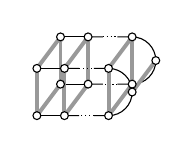
\begin{tikzpicture}
	\dynkin[name=1]A{IIIb}
	\node (a) at (-.3,-.4){};
	\dynkin[name=2,at=(a)]A{IIIb}
	\begin{pgfonlayer}{Dynkin behind}
		\foreach \i in {1,...,7}{
			\draw[/Dynkin diagram/fold style] 
				($(1 root \i)$) -- ($(2 root \i)$);}
	\end{pgfonlayer}
\end{tikzpicture}
\end{tcblisting}
\begin{tcblisting}{}
\pgfkeys{/Dynkin diagram,
    edge length=.75cm,
    edge/.style={draw=example-color,double=black,very thick}}
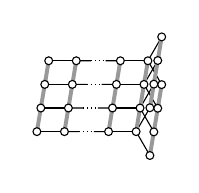
\begin{tikzpicture}
	\foreach \d in {1,...,4}{
		\node (current) at ($(\d*.05,\d*.3)$){};
		\dynkin[name=\d,at=(current)]D{oo.oooo}}
	\begin{pgfonlayer}{Dynkin behind}
		\newcommand\df[2]{
			\draw[/Dynkin diagram/fold style] 
			($(#1 root \i)$) -- ($(#2 root \i)$);}
		\foreach \i in {1,...,6}{\df{1}{2}\df{2}{3}\df{3}{4}}
	\end{pgfonlayer}
\end{tikzpicture}
\end{tcblisting}

\section{Other examples}
\begin{filecontents*}{d44.tex}
\tikzset{/Dynkin diagram,
    edge length=1cm,
    fold radius=1cm,
    label,
    label*=true,
    label macro/.code={\alpha_{#1}},
    label macro*/.code={\beta_{#1}}}
\({}^1 D_4\) 4-ply tied straight:
\begin{dynkinDiagram}[ply=4]D[1]%
{****.*****.*****}
    \dynkinFold 01
    \dynkinFold 1{13}
    \dynkinFold{13}{14}
\end{dynkinDiagram}
\({}^1 D_4\) 4-ply tied bending:
\begin{dynkinDiagram}[ply=4,label]D[1]%
{****.*****.*****}
    \dynkinFold1{13}
    \dynkinFold[bend right=65]0{14}
\end{dynkinDiagram}
\end{filecontents*}
\begingroup\input{d44}\endgroup
\VerbatimInput{d44.tex}
Below we draw the Vogan diagrams of some affine Lie superalgebras \cite{Ransingh:2013,Ransingh:unpub}.
\begingroup
\tikzset{/Dynkin diagram,
	edge length=.35cm,
	fold radius=.3cm,
	label macro/.code=\labls{#1},
	label,
	label*=false,
	root radius=.06cm}
\tcbset{text width=10cm}
\NewDocumentCommand\labls{m}%
{%
	\ifcase#1%
		{1}\or%
		{1}\or%
		{2}\or%
		{2}\or%
		{2}\or%
		{2}\or%
		{2}\or%
		{1}\or%
		{1}\or%
		{1}\or%
		{1}\or%
		{1}\or%
		{1}\or%
		\else\typeout{What? `#1'}%
		\fi%
}%
\NewDocumentCommand\lablIt{m}%
{%
	\ifnum#1=0\relax%
		1%
	\else
		2%
	\fi%
}%
\renewcommand{\wdtA}{2cm}
\NewDocumentEnvironment{Category}{m}%
{%
\begin{tcolorbox}[title={\(#1\)},breakable]{}
}%
{%
\end{tcolorbox}
}%
\begin{Category}{\mathfrak{sl}\left(2m|2n\right)^{(2)}}
\begin{tcblisting}{}
\begin{dynkinDiagram}[ply=2,label]{B}[1]{oo.oto.oo}
	\dynkinLabelRoot*71
\end{dynkinDiagram}
\end{tcblisting}
\begin{tcblisting}{}
\dynkin[label]B[1]{oo.oto.oo}
\end{tcblisting}
\begin{tcblisting}{}
\dynkin[ply=2,label]B[1]{oo.Oto.Oo}
\end{tcblisting}
\begin{tcblisting}{}
\dynkin[label]B[1]{oo.Oto.Oo}
\end{tcblisting}
\begin{tcblisting}{}
\dynkin[label]D[1]{oo.oto.ooo}
\end{tcblisting}
\begin{tcblisting}{}
\dynkin[label]D[1]{oO.otO.ooo}
\end{tcblisting}
\begin{tcblisting}{}
\dynkin[label,fold]D[1]{oo.oto.ooo}
\end{tcblisting}
\end{Category}

\begin{Category}{\mathfrak{sl}\left(2m+1|2n\right)^2}
\begin{tcblisting}{}
\dynkin[label]B[1]{oo.oto.oo}
\end{tcblisting}
\begin{tcblisting}{}
\dynkin[label]B[1]{oO.oto.oO}
\end{tcblisting}
\begin{tcblisting}{}
\dynkin[label,fold]B[1]{oo.oto.oo}
\end{tcblisting}
\end{Category}

\begin{Category}{\mathfrak{sl}\left(2m+1|2n+1\right)^2}
\begin{tcblisting}{}
\dynkin[label]D[2]{o.oto.oo}
\end{tcblisting}
\begin{tcblisting}{}
\dynkin[label]D[2]{o.OtO.oo}
\end{tcblisting}
\end{Category}

\begin{Category}{\mathfrak{sl}\left(2|2n+1\right)^{(2)}}
\begin{tcblisting}{}
\dynkin[ply=2,label,double edges]B[1]{oo.Oto.Oo}
\end{tcblisting}
\begin{tcblisting}{}
\dynkin[ply=2,label,double fold]B[1]{oo.Oto.Oo}
\end{tcblisting}
\begin{tcblisting}{}
\dynkin[ply=2,label,double edges]B[1]{oo.OtO.oo}
\end{tcblisting}
\begin{tcblisting}{}
\dynkin[ply=2,label,double fold]B[1]{oo.OtO.oo}
\end{tcblisting}
\end{Category}

\begin{Category}{\mathfrak{sl}\left(2|2n\right)^{(2)}}
\begin{tcblisting}{}
\dynkin[ply=2,label,double edges]D[1]{oo.oto.ooo}
\end{tcblisting}
\begin{tcblisting}{}
\dynkin[ply=2,label,double fold left]D[1]{oo.oto.ooo}
\end{tcblisting}
\end{Category}

\begin{Category}{\mathfrak{osp}\left(2m|2n\right)^{(2)}}
\begin{tcblisting}{}
\dynkin[label,label macro/.code={1}]D[2]{o.oto.oo}
\end{tcblisting}
\begin{tcblisting}{}
\dynkin[label,label macro/.code={1}]D[2]{o.Oto.Oo}
\end{tcblisting}
\end{Category}

\begin{Category}{\mathfrak{osp}\left(2|2n\right)^{(2)}}
\begin{tcblisting}{}
\dynkin[label,label macro/.code=\lablIt{#1},
	affine mark=*]
	D[2]{o.o.o.o*}
\end{tcblisting}
\begin{tcblisting}{}
\dynkin[label,label macro/.code=\lablIt{#1},
	affine mark=*]
	D[2]{o.O.o.o*}
\end{tcblisting}
\end{Category}

\begin{Category}{\mathfrak{sl}\left(1|2n+1\right)^{4}}
\begin{tcblisting}{}
\dynkin[label,label macro/.code={1}]D[2]{o.o.o.o*}
\end{tcblisting}
\begin{tcblisting}{}
\dynkin[label,label macro/.code={1}]D[2]{o.o.O.o*}
\end{tcblisting}
\end{Category}


\begin{Category}{A^1}
\begin{tcblisting}{}
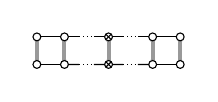
\begin{tikzpicture}
	\dynkin[name=upper]A{oo.t.oo}
	\node (Dynkin current) at (upper root 1){};
	\dynkinSouth
	\dynkin[at=(Dynkin current),name=lower]A{oo.t.oo}
	\begin{pgfonlayer}{Dynkin behind}
	\foreach \i in {1,...,5}{
		\draw[/Dynkin diagram/fold style] 
			($(upper root \i)$) -- ($(lower root \i)$);
	}
	\end{pgfonlayer}
\end{tikzpicture}
\end{tcblisting}
\begin{tcblisting}{}
\dynkin[fold]A[1]{oo.t.ooooo.t.oo}
\end{tcblisting}
\begin{tcblisting}{}
\dynkin[fold,affine mark=t]A[1]{oo.o.ootoo.o.oo}
\end{tcblisting}
\begin{tcblisting}{}
\dynkin[affine mark=t]A[1]{o*.t.*o}
\end{tcblisting}
\end{Category}

\begin{Category}{B^1}
\begin{tcblisting}{}
\dynkin[affine mark=*]A[2]{o.oto.o*}
\end{tcblisting}
\begin{tcblisting}{}
\dynkin[affine mark=*]A[2]{o.oto.o*}
\end{tcblisting}
\begin{tcblisting}{}
\dynkin[affine mark=*]A[2]{o.ooo.oo}
\end{tcblisting}
\begin{tcblisting}{}
\dynkin[odd]A[2]{oo.*to.*o}
\end{tcblisting}
\begin{tcblisting}{}
\dynkin[odd,fold]A[2]{oo.oto.oo}
\end{tcblisting}
\begin{tcblisting}{}
\dynkin[odd,fold]A[2]{o*.oto.o*}
\end{tcblisting}
\end{Category}

\begin{Category}{D^1}
\begin{tcblisting}{}
\dynkin D{otoo}
\end{tcblisting}
\begin{tcblisting}{}
\dynkin D{ot*o}
\end{tcblisting}
\begin{tcblisting}{}
\dynkin[fold]D{otoo}
\end{tcblisting}
\end{Category}

\begin{Category}{C^1}
\begin{tcblisting}{}
\dynkin[double edges,fold,affine mark=t,odd]A[2]{to.o*}
\end{tcblisting}
\begin{tcblisting}{}
\dynkin[double edges,fold,affine mark=t,odd]A[2]{t*.oo}
\end{tcblisting}
\end{Category}

\begin{Category}{F^1}
\begin{tcblisting}{}
\begin{dynkinDiagram}A{oto*}%
	\dynkinQuadrupleEdge 12%
	\dynkinTripleEdge 43%
\end{dynkinDiagram}%
\end{tcblisting}
\begin{tcblisting}{}
\begin{dynkinDiagram}A{*too}%
	\dynkinQuadrupleEdge 12%
	\dynkinTripleEdge 43%
\end{dynkinDiagram}%
\end{tcblisting}
\end{Category}

\begin{Category}{G^1}
\begin{tcblisting}{}
\begin{dynkinDiagram}A{ot*oo}%
	\dynkinQuadrupleEdge 12%
	\dynkinDefiniteDoubleEdge 43%
\end{dynkinDiagram}%
\end{tcblisting}
\begin{tcblisting}{}
\begin{dynkinDiagram}A{oto*o}%
	\dynkinQuadrupleEdge 12%
	\dynkinDefiniteDoubleEdge 43%
\end{dynkinDiagram}%
\end{tcblisting}
\begin{tcblisting}{}
\begin{dynkinDiagram}A{*too*}%
	\dynkinQuadrupleEdge 12%
	\dynkinDefiniteDoubleEdge 43%
\end{dynkinDiagram}%
\end{tcblisting}
\begin{tcblisting}{}
\begin{dynkinDiagram}A{*tooo}%
	\dynkinQuadrupleEdge 12%
	\dynkinDefiniteDoubleEdge 43%
\end{dynkinDiagram}%
\end{tcblisting}
\end{Category}
\endgroup

\section{Example: the complex simple Lie algebras}
\begin{filecontents*}{simple-lie-algebras.tex}
\NewDocumentEnvironment{bunch}{}{
    \renewcommand*{\arraystretch}{1}
    \begin{array}{@{}ll@{}}
    \\ \midrule
}{
    \\ \midrule\end{array}}
\small
\NewDocumentCommand\nct{mm}{
    \newcolumntype{#1}{>{\columncolor[gray]{.9}}>{$}m{#2cm}<{$}}}
\nct{G}{.3}\nct{J}{2.1}\nct{K}{3}\nct{R}{3.7}\nct{S}{3}
\NewDocumentCommand\LieG{}{\mathfrak{g}}
\NewDocumentCommand\W{om}{
    \ensuremath{
        \mathbb{Z}^{#2}
        \IfValueT{#1}{/\left<#1\right>}}}
\renewcommand*{\arraystretch}{1.5}
\NewDocumentCommand\quo{}{\text{quotient of } E_8}
\begin{longtable}{@{}GJKRS@{}}
\LieG&
    \text{Diagram}&
    \text{Weights}&
    \text{Roots}&
    \text{Simple roots}\\ 
\midrule\endfirsthead
\LieG&
    \text{Diagram}&
    \text{Weights}&
    \text{Roots}&
    \text{Simple roots}\\ 
\midrule\endhead
A_n&
    \dynkin A{}&
    \frac1{n+1}\W[\sum e_j]{n+1}&
    e_i-e_j&
    e_i-e_{i+1}\\
B_n&
    \dynkin B{}&
    \frac12\W n&
    \pm e_i, \pm e_i \pm e_j, i\ne j&
    e_i-e_{i+1}, e_n\\
C_n&
    \dynkin C{}&
    \W n&
    \pm 2 e_i, \pm e_i \pm e_j, i\ne j&
    e_i-e_{i+1}, 2e_n\\
D_n&
    \dynkin D{}&
    \frac12\W n&
    \pm e_i \pm e_j, i\ne j &
    \begin{bunch}
        e_i-e_{i+1},&i\le n-1\\
        e_{n-1}+e_n
    \end{bunch}\\
E_8&
    \dynkin E8&
    \frac12\W 8&
    \begin{bunch}
        \pm2e_i\pm2e_j,&i\ne j,\\ 
        \sum_i(-1)^{m_i}e_i,&\sum m_i \text{ even}
    \end{bunch}&
    \begin{bunch}
        2e_1-2e_2,\\
        2e_2-2e_3,\\
        2e_3-2e_4,\\
        2e_4-2e_5,\\
        2e_5-2e_6,\\
        2e_6+2e_7,\\
        -\sum e_j,\\2e_6-2e_7
\end{bunch}\\
E_7&
    \dynkin E7&
    \frac12\W[e_1-e_2]8&
    \quo&
    \quo\\
E_6&
    \dynkin E6&
    \frac13\W[e_1-e_2,e_2-e_3]8&
    \quo&
    \quo\\
F_4& 
    \dynkin F4&
    \W4&
    \begin{bunch}
        \pm 2e_i,\\ 
        \pm 2e_i \pm 2e_j, \quad i \ne j,\\ 
        \pm e_1 \pm e_2 \pm e_3 \pm e_4
    \end{bunch}&
    \begin{bunch}
        2e_2-2e_3,\\
        2e_3-2e_4,\\
        2e_4,\\
        e_1-e_2-e_3-e_4
    \end{bunch}\\
G_2&
    \dynkin G2&
    \W[\sum e_j]3&
    \begin{bunch}
        \pm(1,-1,0),\\ 
        \pm(-1,0,1),\\ 
        \pm(0,-1,1),\\ 
        \pm(2,-1,-1),\\ 
        \pm(1,-2,1),\\ 
        \pm(-1,-1,2)
    \end{bunch}
&
    \begin{bunch}
        (-1,0,1),\\
        (2,-1,-1)
    \end{bunch}
\end{longtable}
\end{filecontents*}
\begingroup
\tikzset{/Dynkin diagram,label macro/.code={},label=false,root radius=.04cm}
\input{simple-lie-algebras.tex}
\endgroup
\VerbatimInput{simple-lie-algebras.tex}

\section{An example of Mikhail Borovoi}
\begin{filecontents*}{borovoi.tex}
\tikzset{
    big arrow/.style={
        -Stealth,
        line cap=round,
        line width=1mm,
        shorten <=1mm,
        shorten >=1mm}}
\newcommand\catholic[2]{
    \draw[big arrow,green!25!white] (root #1) to (root #2);}
\newcommand\protestant[2]{
    \begin{scope}[transparency group, opacity=.25]
        \draw[big arrow,orange] (root #1) to (root #2);
    \end{scope}}
\begin{dynkinDiagram}[%
    edge length=1.2cm,
    indefinite edge/.style={
        thick,
        loosely dotted},
    labels*={0,1,2,3,\ell-3,\ell-2,\ell-1,\ell}]
    D[1]{}
    \catholic 06\catholic 17
    \protestant 70\protestant 61
\end{dynkinDiagram}
\end{filecontents*}
\begingroup
\begin{center}
\input{borovoi.tex}
\end{center}
\endgroup
\VerbatimInput{borovoi.tex}

There are many undocumented features, which are not usually very useful; here is a taste, from \cite{Humphreys:1978} p. 61.

\begin{filecontents*}{humphreys.tex}
\begin{center}
\makeatletter
\newcommand{\extraNode}[6]%
{%
\dynkinPlaceRootRelativeTo{#1}{#2}{#3}{#4}{#5}
\dynkinDefiniteSingleEdge{#1}{#2}
\dynkinRootMark{o}{#1}
\advance\dynkin@nodes by 1
\dynkinLabelRoot{#1}{#6} 
}%
\newcommand{\extraDotNode}[6]%
{%
\dynkinPlaceRootRelativeTo{#1}{#2}{#3}{#4}{#5}
\dynkinIndefiniteSingleEdge{#1}{#2}
\dynkinRootMark{o}{#1}
\advance\dynkin@nodes by 1
\dynkinLabelRoot{#1}{#6} 
}%
\makeatother
\tikzset{/Dynkin diagram,mark=o,edge length=.5cm}
\begin{tabular}{>{\columncolor[gray]{.9}}c}
\dynkin A{}
\\ \midrule
\begin{dynkinDiagram}A{ooo.o}
\dynkinLabelRoot{1}{\varepsilon_1}
\dynkinLabelRoot{2}{\varepsilon_2}
\dynkinLabelRoot{3}{\varepsilon_3}
\dynkinLabelRoot{4}{\varepsilon_p}
\dynkin[at=(root 4),arrows=false]B2
\dynkin[at=(root 2),labels={\eta_q,\eta_{q-1},\eta_2,\eta_1}]A{oo.oo}
\end{dynkinDiagram}
\\ \midrule
\dynkin[arrows=false] G{2}
\\ \midrule
\begin{dynkinDiagram}[%
labels={\varepsilon_{p-1},\psi,\zeta_{r-1},\eta_{q-1}},
mark=o,edge length=.75cm]D4
\extraDotNode{5}{3}{northeast}{right}{left}{\zeta_2}
\extraDotNode{6}{4}{southeast}{right}{left}{\eta_2}
\extraDotNode{7}{1}{west}{below}{above}{\varepsilon_2}
\extraNode{8}{5}{northeast}{right}{left}{\zeta_1}
\extraNode{9}{6}{southeast}{right}{left}{\eta_1}
\extraNode{10}{7}{west}{below}{above}{\varepsilon_1}
\end{dynkinDiagram}
\end{tabular}
\end{center}
\end{filecontents*}
\begingroup
\tikzset{/Dynkin diagram,label=false,label*=false}
\input{humphreys.tex}
\endgroup
\VerbatimInput[commentchar=!]{humphreys.tex}


\section{Syntax}
The syntax is \verb!\dynkin[<options>]{<letter>}[<twisted rank>]{<rank>}! where \verb!<letter>! is \verb!A!, \verb!B!, \verb!C!, \verb!D!, \verb!E!, \verb!F! or \verb!G!, the family of root system for the Dynkin diagram, \verb!<twisted rank>! is \verb!0!, \verb!1!, \verb!2!, \verb!3! (default is \verb!0!) representing:
\[
\renewcommand*{\arraystretch}{1}
\begin{array}{rp{8cm}}
0 & finite root system \\ \hline
1 & affine extended root system, i.e.  of type \({}^{(1)}\) \\
2 & affine twisted root system of type \({}^{(2)}\) \\
3 & affine twisted root system of type \({}^{(3)}\) \\
\end{array}
\]
and \verb!<rank>! is 
\begin{enumerate}
\item
an integer representing the rank or 
\item
blank to represent an indefinite rank or
\item
the name of a Satake diagram as in section~\ref{section:Satake}.
\end{enumerate}
The environment syntax is \verb!\begin{dynkinDiagram}! followed by the same parameters as \verb!\dynkin!, then various Dynkin diagram and \TikZ{} commands, and then \verb!\end{dynkinDiagram}!.

\section{Options}
\newcommand*{\typ}[1]{\(\left<\texttt{#1}\right>\)}
\newcommand{\TikZstyle}{\TikZ style data}
\newcommand{\truefalse}{{\texttt{true}}\ or {\texttt{false}}}
\newcommand{\notset}{\textrm{not set}}

\newcommand*{\optionLabel}[3]{%%
\multicolumn{2}{l}{\(\texttt{#1}=\textrm{#2}\),} \\
\multicolumn{2}{l}{\(\textrm{default}: \texttt{#3}\)} \\
}%%
\renewcommand*{\arraystretch}{1}
\par\noindent%
\begin{longtable}{p{1cm}p{10cm}}
\endfirsthead
\caption{\dots continued}\\
\endhead
\multicolumn{2}{c}{continued \dots}\\
\endfoot
\endlastfoot
\optionLabel{*/.style}{\TikZstyle}{solid,draw=black,fill=black}
& style for roots like \dynkin{A}{*} \\
\optionLabel{o/.style}{\TikZstyle}{solid,draw=black,fill=white}
& style for roots like \dynkin{A}{o}  \\
\optionLabel{O/.style}{\TikZstyle}{solid,draw=black,fill=white}
& style for roots like \dynkin{A}{O}  \\
\optionLabel{t/.style}{\TikZstyle}{solid,draw=black,fill=black}
& style for roots like \dynkin{A}{t} \\
\optionLabel{x/.style}{\TikZstyle}{solid,draw=black,line cap=round}
& style for roots like \dynkin{A}{x}  \\
\optionLabel{X/.style}{\TikZstyle}{solid,draw=black,thick,line cap=round}
& style for roots like \dynkin{A}{X} \\
\optionLabel{affine mark}{o,O,t,x,X,*}{*}
&      default root mark for root zero in an affine Dynkin diagram \\
\optionLabel{arrow shape/.style}{\TikZstyle}{-\{Computer Modern Rightarrow[black]\}}
&      shape of arrow heads for most Dynkin diagrams that have arrows\\
\optionLabel{arrow style}{\TikZstyle}{black}
& set to override the default style for the arrows in nonsimply laced Dynkin diagrams, including length, width, line width and color  \\
\optionLabel{arrow width}{length}{1.5(root radius)}
& if you change arrow style or shape, use \texttt{arrow width} to say how wide your arrows will be \\
\optionLabel{arrows}{\truefalse}{true}
& whether to draw the arrows that arise along the edges \\
\optionLabel{backwards}{\truefalse}{false}
& whether to reverse right to left \\
\optionLabel{bird arrow}{\truefalse}{false}
& whether to use bird style arrows in \(G_2,F_4\).\\
\optionLabel{Bourbaki arrow}{\truefalse}{false}
& whether to use Bourbaki style arrows in \(G_2,F_4\). \\
\optionLabel{ceref}{\truefalse}{false}
&      whether to draw roots in a ``ceref'' style \\
\optionLabel{Coxeter}{\truefalse}{false}
& whether to draw a Coxeter diagram, rather than a Dynkin diagram \\
\optionLabel{double edges}{\TikZstyle}{\notset}
& set to override the \texttt{fold} style when folding roots together in a Dynkin diagram, so that the foldings
are indicated with double edges (like those of an \(F_4\) Dynkin diagram without arrows) \\
\optionLabel{double fold}{\TikZstyle}{\notset}
& set to override the \texttt{fold} style when folding roots together in a Dynkin diagram, so that the foldings
are indicated with double edges (like those of an \(F_4\) Dynkin diagram without arrows), but filled in solidly \\
\optionLabel{double left}{\TikZstyle}{\notset}
& set to override the \texttt{fold} style when folding roots together at the left side of a Dynkin diagram, so that the foldings are indicated with double edges (like those of an \(F_4\) Dynkin diagram without arrows) \\
\optionLabel{double fold left}{\TikZstyle}{\notset}
& set to override the \texttt{fold} style when folding roots together at the left side of a Dynkin diagram, so that the foldings are indicated with double edges (like those of an \(F_4\) Dynkin diagram without arrows), but filled in solidly \\
\optionLabel{double right}{\TikZstyle}{\notset}
& set to override the \texttt{fold} style when folding roots together at the right side of a Dynkin diagram, so that the foldings are indicated with double edges (like those of an \(F_4\) Dynkin diagram without arrows) \\
\optionLabel{double fold right}{\TikZstyle}{\notset}
& set to override the \texttt{fold} style when folding roots together  at the right side of a Dynkin diagram, so that the foldings are indicated with double edges (like those of an \(F_4\) Dynkin diagram without arrows), but filled in solidly\\
\optionLabel{edge label/.style}{\TikZstyle}{text height=0,text depth=0,label distance=-2pt}
&      style of edge labels in the Dynkin diagram, as found, for example, on some Coxeter diagrams \\
\optionLabel{edge length}{length}{.35cm}
&      distance between nodes in the Dynkin diagram \\
\optionLabel{edge/.style}{\TikZstyle}{solid,draw=black,fill=white,thin}
&      style of edges in the Dynkin diagram \\
\optionLabel{extended}{\truefalse}{false}
&      Is this an extended Dynkin diagram? \\
\optionLabel{fold}{\truefalse}{true}
& whether, when drawing Dynkin diagrams, to draw them 2-ply\\
\optionLabel{fold left}{\truefalse}{true}
& whether to fold the roots on the left side of a Dynkin diagram\\
\optionLabel{fold radius}{length}{.3cm}
& the radius of circular arcs used in curved edges of folded Dynkin diagrams\\
\optionLabel{fold right}{\truefalse}{true}
& whether to fold the roots on the right side of a Dynkin diagram\\
\optionLabel{fold left style/.style}{\TikZstyle}{}
& style to override the \texttt{fold} style when folding roots together on the left half of a Dynkin diagram \\
\optionLabel{fold right style/.style}{\TikZstyle}{}
& style to override the \texttt{fold} style when folding roots together on the right half of a Dynkin diagram \\
\optionLabel{fold style/.style}{\TikZstyle}{solid,draw=black!40,fill=none,line width=radius}
& when drawing folded diagrams, style for the fold indicators\\
\optionLabel{gonality}{math}{0}
& the gonality of a \(G\) or \(I\) Coxeter diagram \\
\optionLabel{horizontal shift}{length}{0}
& the gonality of a \(G\) or \(I\) Coxeter diagram \\
\optionLabel{indefinite edge ratio}{float}{1.6}
& ratio of indefinite edge lengths to other edge lengths\\
\optionLabel{indefinite edge/.style}{\TikZstyle}{solid,draw=black,fill=white,thin,densely dotted}
& style of the dotted or dashed middle third of each indefinite edge\\
\optionLabel{involution/.style}{\TikZstyle}
{latex-latex,black} & style of involution arrows\\
\optionLabel{involutions}{semicolon separated list of pairs}
{} & involution double arrows to draw\\
\optionLabel{Kac}{\truefalse}{false}
& whether to draw in the style of \cite{Kac:1990} \\
\optionLabel{Kac arrows}{\truefalse}{false}
& whether to draw arrows in the style of \cite{Kac:1990} \\
\optionLabel{label}{\truefalse}{false}
& whether to label the roots according to the current labelling scheme\\
\optionLabel{label*}{\truefalse}{false}
& whether to label the roots at alterative label locations according to the current labelling scheme\\
\optionLabel{label depth}{1-parameter \TeX{} macro}{g}
& the current maximal depth of text labels for the roots, set by giving mathematics text of that depth\\
\optionLabel{label directions}{comma separated list}{}
& list of directions to place root labels: above, below, right, left, below right, and so on. \\
\optionLabel{label* directions}{comma separated list}{}
& list of directions to place alternate root labels: above, below, right, left, below right, and so on. \\
\optionLabel{label height}{\typ{1-parameter \TeX{} macro}}{b}
& the current maximal height of text labels for the roots, set by giving mathematics text of that height\\
\optionLabel{label macro}{1-parameter \TeX{} macro}{\texttt{\#1}}
& the current labelling scheme for roots\\
\optionLabel{label macro*}{\typ{1-parameter \TeX{} macro}}{\texttt{\#1}}
& the current labelling scheme for alternate roots\\
\optionLabel{make indefinite edge}{\typ{edge pair \(i\)-\(j\) or list of such}}{\{\}}
& edge pair or list of edge pairs to treat as having indefinitely many roots on them\\
\optionLabel{mark}{\typ{o,O,t,x,X,*}}{*}
&      default root mark \\
\optionLabel{name}{\typ{string}}{anonymous}
& A name for the Dynkin diagram, with \texttt{anonymous} treated as a blank; see section~\ref{section:name}\\
\optionLabel{ordering}{\typ{Adams, Bourbaki, Carter, Dynkin, Kac}}{Bourbaki}
& which ordering of the roots to use in exceptional root systems as in section~\ref{section:order}\\
\optionLabel{parabolic}{\typ{integer}}{0} 
& A parabolic subgroup with specified integer, where the integer
is computed as \(n=\sum 2^{i-1} a_i\), \(a_i=0\) or \(1\), to say that root \(i\) is crossed, i.e. a noncompact root\\
\optionLabel{ply}{\typ{0,1,2,3,4}}{0}
& how many roots get folded together, at most\\
\optionLabel{reverse arrows}{\truefalse}{true}
& whether to reverse the direction of the arrows that arise along the edges\\
\optionLabel{root radius}{\typ{number}cm}{.05cm}
&      size of the dots and of the crosses in the Dynkin diagram \\
\optionLabel{separator length}{length}{.35cm}
&      distance between successive components of a disconnected Dynkin diagram \\
\optionLabel{text style}{\TikZstyle}{scale=.7}
& Style for any labels on the roots\\
\optionLabel{upside down}{\truefalse}{false}
& whether to reverse up to down\\
\optionLabel{vertical shift}{\typ{length}}{.5ex}
& amount to shift up the Dynkin diagram, from the origin of \TikZ coordinates.\\
\end{longtable}
\par\noindent{}All other options are passed to TikZ.
To force addition expansion, you can add the word \verb!expand! in front of
\par\noindent
{
\centering
\begin{tabular}{>{\ttfamily}l}
affine mark\\
arrow color\\
arrow style\\
arrow width\\
at\\
edge length\\
fold radius\\
gonality\\
involutions\\
label directions\\
label* directions\\
labels\\
labels*\\
mark\\
name\\
ordering\\
parabolic\\
ply\\
root radius\\
separator length\\
twisted series\\
vertical shift
\end{tabular}

}


\nocite{*}
\bibliographystyle{amsplain}
\bibliography{dynkin-diagrams}
\end{document}
